\documentclass[letterpaper,10pt,onecolumn]{article}
\usepackage[spanish]{babel}
\usepackage[utf8x]{inputenc}
\usepackage{amsfonts}
\usepackage{amsthm}
\usepackage{amsmath}
\usepackage{mathrsfs}
\usepackage{empheq}
\usepackage{enumitem}
\usepackage[pdftex]{color,graphicx}
\usepackage{hyperref}
\usepackage{listings}
\usepackage{calligra}
\usepackage{algpseudocode} 
\DeclareMathAlphabet{\mathcalligra}{T1}{calligra}{m}{n}
\DeclareFontShape{T1}{calligra}{m}{n}{<->s*[2.2]callig15}{}
\newcommand{\scripty}[1]{\ensuremath{\mathcalligra{#1}}}
\lstloadlanguages{[5.2]Mathematica}
\setlength{\oddsidemargin}{0cm}
\setlength{\textwidth}{490pt}
\setlength{\topmargin}{-40pt}
\addtolength{\hoffset}{-0.3cm}
\addtolength{\textheight}{4cm}

\begin{document}
\begin{center}



\includegraphics[width=490pt]{header.png}\\[0.5cm]

\textsc{\LARGE Taller 6 - F\'isica I (FISI-1018) - 2016-10}\\[0.5cm]

\textsc{\Large{Profesor: Jaime Forero}} \\[0.5cm]

\noindent\textsc{Ejercicios correspondiente a la clase complementaria de la semana del 29 de Febrero del 2016.}\\[0.5cm]
\end{center}

\noindent\textsc{Nota:} 
Los primeros tres ejercicios deben ser
entregados {\bf al comienzo} de la clase complementaria. Los \'ultimos
cuatro deben ser trabajados {\bf durante} la complementaria. 

La numeraci\'on
hace referencia al texto gu\'ia: \textit{F\'isica Universitaria Volumen
  1 (Sears-Semansky)}, decimotercera edici\'on, Pearson.

\begin{enumerate}
% aqui vienen los tres ejercicios "faciles"
\item Ejercicio 5.14 (Tres botes) %Juan Carlos

\item
En la figura se ilustra  el sistema de poleas denominado  Maquina de Atwood, encuentre la aceleración de cada una de las masas y la tensión en la cuerda. 
\begin{figure}[h]
\begin{center} 
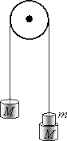
\includegraphics[scale=0.80]{maquinadeatwood.png} 
\end{center} 
\end{figure}
  
\item \label{adulto}Un adulto de masa $M$ sostiene a un ni\~no de masa $m$ con una
  cuerda a trav\'es de una polea como se muestra en la
  Figura \ref{fig:adulto}. Cu\'anto vale la normal que hace el piso sobre el adulto si
  $M=70$kg y $m=$20kg?
\begin{figure}[h]
\begin{center} 
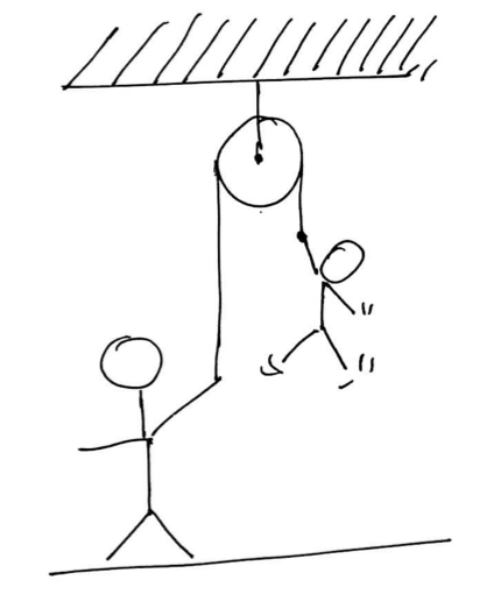
\includegraphics[scale=0.25]{adulto.png} 
\caption{\label{fig:adulto}Figure para el problema \ref{adulto}}
\end{center} 
\end{figure}



% aqui vienen los cuatro ejercicios "dificiles"
\item Ejercicio 5.97 (Un bloque sostenido por un carro en movimiento) %Juan Carlos

\item\label{bloques} %Jaime
Tenemos la configuraci\'on de bloques mostrada en la Figura \ref{fig:bloques}. 
Entre los bloques hay fricci\'on con coeficiente est\'atico $\mu$, pero entre los bloques y el piso no hay fricci\'on. Encuentre la fuerza m\'axima $F$ que se puede hacer antes de que el bloque $m_1$ a la derecha empieze a deslizarse sobre el bloque $m_2$

\begin{figure}[h]
\begin{center} 
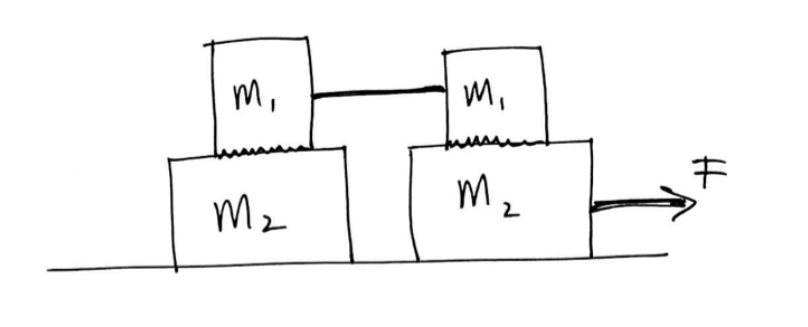
\includegraphics[scale=0.25]{bloques.png} 
\caption{\label{fig:bloques}Figure para el problema \ref{bloques}}
\end{center} 
\end{figure}


%Miguel
\item
Encuentre la aceleración del sistema y la tensión en la cuerda siguiendo el procedimiento que se muestra a continuación:
\begin{figure}[h]
\begin{center} 
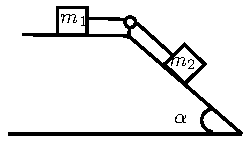
\includegraphics{complementaria11.pdf} 
\end{center} 
\end{figure}

\begin{enumerate}
\item
Realice los diagramas de cuerpo libre para $m_1$ y $m_2$.
\item
Para cada diagrama plantee las respectivas ecuaciones de Newton.
\item
Despeje la aceleración del sistema de ecuaciones (Sugerencia: elimine la tensión)
\item
sustituya la aceleración en una ecuación que le permita hallar la tensión
\item
Asuma que $m_1=10kg$,  $m_2=20kg$ y $\alpha=60^{\circ}$, cuanto valdría la aceleración y la tensión en este caso. 
 \end{enumerate}
 
 \item \label{conico} Una cuerda sin masa y de longitud $l$ tiene en su extremo una masa $m$. Con esto se arma un p\'endulo c\'onico como muestra la Figura \ref{fig:conico}. La m\'axima tensi\'on que puede soportar la cuerda es
  $2mg$. Cu\'anto es la velocidad m\'axima que puede tener la masa antes de que se rompa la cuerda si $m=1$kg y $l=1$m?
 \begin{figure}[h]
\begin{center} 
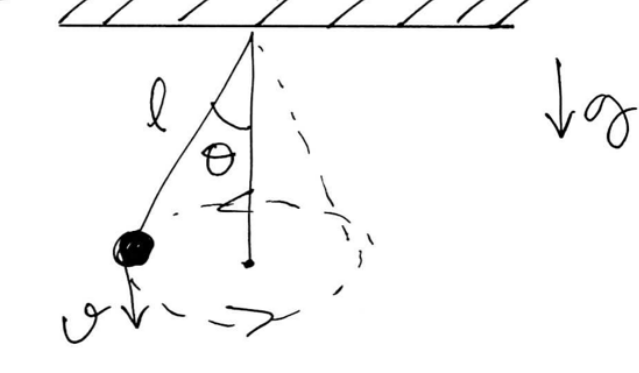
\includegraphics[scale=0.25]{conico.png} 
\caption{\label{fig:conico}Figure para el problema \ref{conico}}
\end{center} 
\end{figure}
%Miguel
\end{enumerate}

\end{document}

\begin{figure}[!h]
\begin{center}
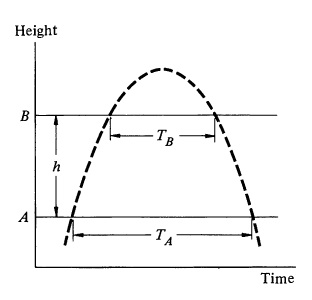
\includegraphics[scale=0.7]{altura.jpg} 
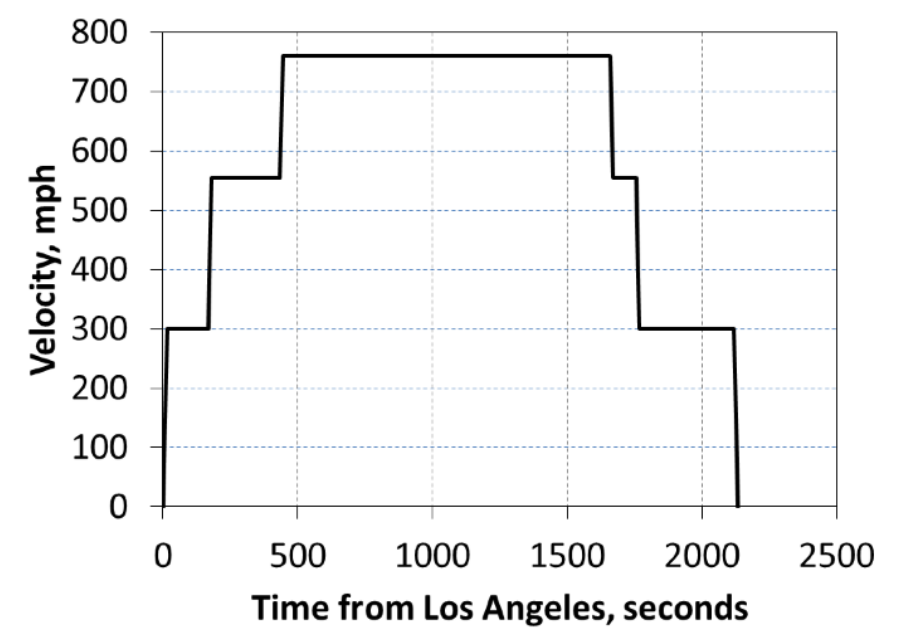
\includegraphics[scale=0.3]{hyperloop.png} 
\end{center}
\caption{Izquierda: diagrama para el ejercicio recomendado 3. Derecha: diagrama para el ejercicio recomendado 4.}
\label{fig:tiro}
\end{figure}





